\begin{eg}
   \begin{enumerate}
       \item $E = \R$, \quad  $d(x, y) = |x - y|$
            \[
                B(x_0, r) = ]x_0 -r, x_0 + r[
           \] 
       \item $E = \R^d$, \quad $d = 2,3$, \quad $X = (x_1, \ldots, x_d)$ 
           \begin{align*}
               &\|X\|_2 = \left( \sum_{i=1}^{d} x_i^2 \right)^{\frac{1}{2}} \\
               &\|X\|_1 = \sum_{i=1}^{d} x_i\\
               &\|X\|_{\infty} = \underset{1 \le i \le d}{\text{max}}|x_i|
           \end{align*}
           \begin{align*}
              &d_2(X, Y) = \|Y - X\|_2 = \|\vec{XY}\|_2\\ 
              &d_1(X, Y), d_{\infty}(X, Y)
           \end{align*}
   \end{enumerate} 
\end{eg}
\begin{property} Dans $\R^n$
   \begin{itemize}
       \item $d_{\infty}(X, Y) \le d_1(X, Y) \le n d_{\infty}(X, Y)$
       \item $d_{\infty}(X, Y) \le d_2(X, Y) \le \sqrt{n} d_{\infty}(X, Y)$
   \end{itemize} 
\end{property}
\section{Parties bornées de $(E, d)$}
\begin{definition}
    Soit $A \subset E$. $A$ est bornée si  $\exists R > 0$ et $\exists x_0 \in E$ tel que 
    \[
    A \subset B(x_0, R)
    \] 
\end{definition}
\begin{figure}[H]
    \centering
    \incfig{exemple-bornee}
    \caption{Exemple d'un enesemble borné}
    \label{fig:exemple-bornee}
\end{figure}
\begin{lemma}
   Les propriétés suivantes sont équivalentes:
   \begin{enumerate}
       \item $A$ est bornée
       \item  $\forall x_0 \in E, \exists r > 0$ tel que $A \subset B(x_0, r)$
       \item $\exists r > 0$ tel que $\forall x, y \in A$ on a $d(x, y) < r$
   \end{enumerate}
\end{lemma}
\begin{explanation} de lemme
   \begin{itemize}
       \item $(1) \implies (2)$ :\\
           \underline{Hyp}: $\exists x_1 \in E, \exists r_1 \in E$ tq $A \subset B(x_1, r_1)$\\
           Soit $x_0 \in E$. But: trouver $r$ tel que  $A \subset B(x_0, r)$ si $x \in A$, on a:  $d(x_1, x) < r_1$\\
           \underline{Je veux}: $d(x_0, x) <r$\\
          \begin{align*}
              d(x_0, x) \le d(x_0, x_1) + d(x_1, x) \le d(x_0, x_1) + r_1 < r \quad \text{ si } r > d(x_0, x_1) + r_1
          \end{align*} 
   \end{itemize} 
\end{explanation}
\begin{property}
   \begin{enumerate}
       \item Toute partie finie est bornée
       \item Si $A$ bornée et  $B \subset A$ alors $B$ bornée
       \item L'union d'un nombre \underline{fini} de bornés est borné
   \end{enumerate} 
\end{property}
\begin{preuve}{de (3).}\\
    $A_1, \ldots, A_n$ sont bornés. \underline{Je fixe $x_0 \in E$}, $A_i$ borné ($1 \le i \le n$), donc $\exists r_i > 0$ tel que $A_i \subset B(x_0, r_i)$ si $r = \underset{1 \le  i \le n}{max} r_i$ 
    \[
        A_i \subset B(x_0, r), \, \forall i \implies \bigcup\limits_{i=1}^{n} A_i \subset B(x_0, r)
    \] 
\end{preuve}
\section{Fonctions bornées}
\begin{definition}
    Soit $B$ un ensemble. Une fonction  $F: B \to E$ est bornée si $F(B) = \{ F(b): b \in B\} \subset E$ est borné.
\end{definition}
\section{Distance entre ensembles}
\begin{definition}
    La distance entre deux ensembles $A, B$ est:
     \[
         d(A, B) := \underset{x \in A, y \in B}{inf}d(x, y)
    \] 
    Intuitivement, on cherche deux points $x$ et  $y$ tel que la distance est la plus petite possible.
\end{definition}
\begin{definition}
    La distance entre un points $x$ et un ensemble  $B$ est:
     \[
         d(x, B) := \underset{y \in B}{inf}d(x, y)
    \] 
    La même intuition.
\end{definition}
\begin{property}
   $\forall x \in A, \, y \in B, \, d(x, y) \ge d(A, B)$ et $\forall \epsilon > 0, \exists x \in A, \, y \in B$ tq $d(x, y) \le d(A, B) + \epsilon$
\end{property}
\begin{figure}[H]
    \centering
    \incfig{distance-entre-ensembles}
    \caption{Distance entre ensembles}
    \label{fig:distance-entre-ensembles}
\end{figure}
\section{Topologie des espaces métriques}
distance $d(x, y)$ $\longrightarrow$ boules  $B(x_0, r)$ $\longrightarrow$ ensembles ouverts
\begin{definition}
    Soit (E, d) espace métrique.
    \begin{enumerate}
        \item $U \subset E$ est ouvert si $\forall x_0 \in U, \, \exists r > 0 \: r(x_0)$ tel que $B(x_0, r) \subset U$
        \item $F \subset E$ est fermé si $E \setminus F$ est ouvert
    \end{enumerate}
    $\O$ est ouvert et $E$ est ouvert.  $\O$ est fermé et $E$ est fermé.
\end{definition}
\begin{figure}[H]
    \centering
    \begin{subfigure}{0.45\textwidth}
        \centering 
        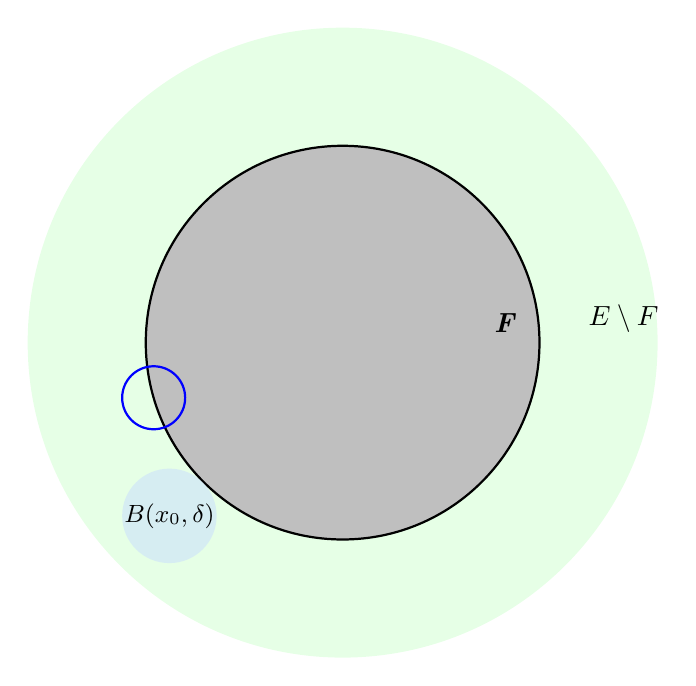
\begin{tikzpicture}
            % Define colors
            \definecolor{lightgreen}{RGB}{230, 255, 230}
            \definecolor{lightblue}{RGB}{200, 220, 255}
            \definecolor{darkgreen}{RGB}{0, 128, 0}

            % Large background circle
            \fill[lightgreen] (0, 0) circle (4cm);

            % Main circle
            \draw[thick, fill=lightgray] (0, 0) circle (2.5cm);
            \node[above right] at (1.8, 0) {\textbf{\textit{F}}};
            \node[above right] at (3, 0) {$E\setminus F$};

            % Small blue circle
            \draw[blue, thick] (-2.4, -.7) circle (0.4cm);

            % Highlighted area for excluded point
            \fill[lightblue, opacity=0.5] (-2.2, -2.2) circle (0.6cm);
            \node (_) at (-2.2, -2.2){\small $B(x_0, \delta)$};
        \end{tikzpicture}
        \caption{Un ensemble fermé\\
            \textit{À la borne, il est impossible de trouver une boules qui appartient à $F$, car il est impossible d'avoir une boule ouverte de  $r = 0$. Exemple: circle bleu foncé}\\
            \textit{Pour tout point dans $E \setminus F$ on peut trouver une boule ouverte}
        }
    \end{subfigure}
    \hfill
    \begin{subfigure}{0.45\textwidth}
        \centering
        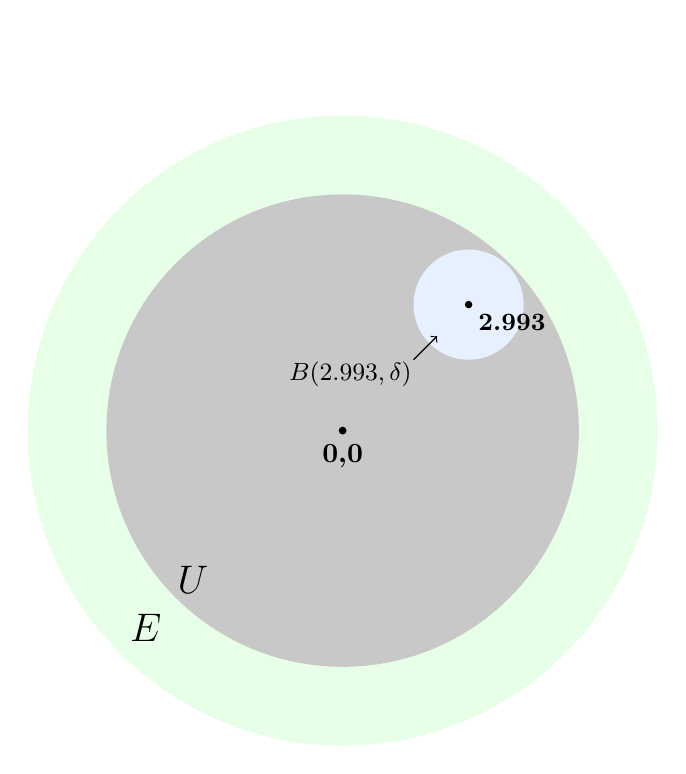
\begin{tikzpicture}
            % Define colors
            \definecolor{lightblue}{RGB}{230, 240, 255}
            \definecolor{lightgray}{RGB}{200, 200, 200}
            \definecolor{darkgreen}{RGB}{0, 128, 0}
            \definecolor{lightgreen}{RGB}{230, 255, 230}

            % Draw large circle
            \fill[lightgreen] (0, 0) circle (4cm);
            \fill[lightgray] (0, 0) circle (3cm);

            % Draw small circle
            \fill[lightblue] (1.6, 1.6) circle (0.7cm);
            \draw[fill=black] (1.6, 1.6) circle(0.4mm);
            \node[below right] at (1.6, 1.6) {\textbf{\small 2.993}};

            \draw[->] (0.9, 0.9)--(1.2, 1.2);
            \node[below left] (_) at (1, 1){\small $B(2.993, \delta)$};
            % Add points and labels
            \node[fill=black, circle, inner sep=1pt, label=below:{\textbf{0,0}}] at (0, 0) {};

            % Add text
            \node[right] at (1, 5) [align=left, text=darkgreen] {
                };
            \node (_) at (-1.9, -1.9){\Large $U$};
            \node (_) at (-2.5, -2.5){\Large $E$};
        \end{tikzpicture} 
        \caption{Un ensemble ouvert\\
            \textit{
                pour tout point pres de la borne
                on peut trouver une boule
                infiniment petite avec des
                points autour ce point inclu dans $U$.
            }
        }

    \end{subfigure}
    \caption{Démonstration des espaces ouverts et fermés}
\end{figure}
\begin{remark}
   dans $\R$ les intervalles ouverts sont des ouverts (pareil pour fermés) 
\end{remark}
\begin{remark}
   Une distance entre deux ensembles ouverts toujours existe et elle est infimum (qui n'est jamais atteint) 
\end{remark}
\begin{lemma}
   \begin{enumerate}
       \item $B(x_0, r_0)$ est ouvert.
       \item $B_f(x_0, r_0)$ est fermé.
   \end{enumerate} 
\end{lemma}
\begin{preuve}
   \begin{enumerate}
       \item Soit $x_1 \in B(x_0, r_0)$ ($d(x_0, x_1) < r_0$).\\
           But: touver $r_1 > 0$ tel que $B(x_1, r_1) \subset B(x_0, r_0)$?\\
           \begin{align*}
               &x \in B(x_1, r_1): \: d(x_1, x) < r_1\\
               &x \in B(x_0, r_0) \text{ si } d(x_0, x) < r_0
           \end{align*}
           facile:
           \begin{align*}
               d(x_0, x) &\le d(x_0, x_1) + d(x_1, x)\\
                         &\le d(x_0, x_1) + r_1\\
                         &< r_0 \text{ si}
           \end{align*}
           $r_1 < r_0 - d(x_0, x_1) > 0$
   \end{enumerate} 
\end{preuve}
\begin{eg} bizzare.\\
    Soit $E = \R$, $d(x, y) = |y - x|$,  $A = ]0, 1[$ ouvert, pas fermé dans  $\R$.\\
    \begin{center}
       \begin{tikzpicture}
          \draw (-2, 0) -- (2, 0); 
          \node (x) at (0, 0){]};
          \node (y) at (1, 0){[};
          \node[below] (x) at (0, -0.2){$0$};
          \node[below] (y) at (1, -0.2){$1$};
          \draw[color=red] (-2, 0) -- (0, 0);
          \draw[color=red] (1, 0) -- (2, 0);
       \end{tikzpicture} 
    \end{center}
    Je regarde $A$ comme partie de  $(A, d)$. Comme  $A \setminus A = \O$ qui est ouvert, donc $A$ est fermé dans $A$. Par contre, les bornes ne sont jamais atteints, alors $A$ est ouvert dans  $(A, d)$.
\end{eg}
\begin{theorem}.
    \begin{enumerate}
        \item Soit $U_i$,  $i \in I$ une collection d'ouverts. Alors,  $\cup_{i \in I} \,U_i$ est ouvert.\\
            Translate: Une union quelconque des ensembles ouverts est ouvert.
        \item Si $U_1, \ldots, U_n$ sont ouverts
            \[
                \bigcap\limits_{i=1}^{n} \, U_i \text{ est ouvert.}
            \] 
            Translate: intersection \underline{finie} des ensembles ouverts est ouvert.
    \end{enumerate}
    \begin{enumerate}
        \item Soit $U_i$,  $i \in I$ une collection de fermés. Alors,  $\cup_{i \in I} \,U_i$ est fermé.\\
            Translate: Une union quelconque des ensembles fermés est fermé.
        \item Si $U_1, \ldots, U_n$ sont fermés 
            \[
                \bigcap\limits_{i=1}^{n} \, U_i \text{ est fermé.}
            \] 
            Translate: intersection \underline{finie} des ensembles fermés est fermé.
    \end{enumerate}
\end{theorem}
\begin{preuve}.
    \begin{enumerate}
        \item Soit $x \in U := \bigcup\limits_{i \in I} U_i$. Il existe un $i$ noté  $i_0$ tel que $x \in U_{i_0}$, $U_{i_0}$ est ouvert, donc $\exists r > 0$ tel que $B(x, r) \subset U_{i_0} \subset U := \bigcup\limits_{i \in I} U_i$.
        \item Soit $x \in U := \bigcap\limits_{1 \le i \le n} U_i$.\\
            On fixe $i$.  $x \in U_i$,  $U_i$ ouvert, donc  $\exists r_i > 0$ tel que $B(x, r) \subset U_i$, $1 \le i \le n$, donc $B(x, r) \subset U := \bigcap\limits_{1 \le i \le n} U_i$
    \end{enumerate}
\end{preuve}

\section{Algorithmes pour montrer qu'un ensemble est ouvert/fermé}
\begin{center}
    
\begin{tabular}{c | c}
    {\large \bf
    Montrer qu'un ensemble est ouvert      } 
 & 
    {\large \bf
    Montrer qu'un ensemble est fermé }
 \\
 \hline
 \parbox[t]{8cm}{
\begin{itemize}
    \item \textbf{Utiliser la définition :} 
    \[
    \forall x \in \mathcal{U}, \exists r > 0 \quad \text{tel que} \quad B(x, r) \subset \mathcal{U}
    \]
    
    \item Montrer que \( E \setminus \mathcal{U} \) est fermé.
    
    \item Montrer que \(\mathcal{U}\) est l'image réciproque d'un ouvert par une application continue.
    
    \item Exprimer \(\mathcal{U}\) comme une boule ouverte.
    
    \item Écrire \(\mathcal{U}\) comme :
    \begin{itemize}
        \item une réunion d'ouverts ;
        \item une intersection finie d'ouverts.
    \end{itemize}
    
    \item \(\mathcal{U} = \operatorname{Int}(U)\).
    
    \item Écrire \(\mathcal{U} = I_1 \times \dots \times I_n\) avec \( I_i \) ouvert.
\end{itemize}
} & \parbox[t]{8cm}{
\begin{itemize}
    \item \textbf{Utiliser la définition :} \( E \setminus V \) est ouvert.
    
    \item \textbf{Caractérisation séquentielle :} Toute suite convergente dans \(V\), sa limite est aussi dans \(V\).
    
    \item Montrer que \(V\) est l'image réciproque d'un fermé par une application continue.
    
    \item Montrer que \(V\) est compact.
\end{itemize}
}
\end{tabular}
\end{center}
